\chapter{Garment Analysis}
\label{garment_analysis}

This chapter explains in detail the gament analysis that our algorithm performs to the garment data previously segmented. The contour of the garment is extracted, and a Watershed segmentation algorithm is applied to find the different overlapped patches.

\section{Contour extraction}
From the mask obtained in the previous step (section \ref{garment_segmentation_mask}) a blob labeling algorithm is applied to detect the garment outline. This outline will be used in later steps to obtain the candidates to be a fold.

The contour extraction method used is the Topological Analysis by Border Following algorithm developed by Suzuki and Abe\comment{[ref to suzuki85]}. This is a widely used algorithm for connected-component labeling and countour finding. Only external contours were retrieved. A simple chain approximation was then applied to reduce the number of points that describe the contours, storing only the endpoints of the different segments.

Due to noise, sometimes some small blobs appear in segmentation masks, so the extracted contour with the highest area was selected as garment. This way, those small blobs were discarded.
After obtaining the garment contour, it is processed, as we want to obtain a further simplified garment outline. We assume the fold line has a very high probability of lying in the garment outline and, therefore, this contour will represent all the candidate segments to be a fold. 

To obtain the simplified outline, the Ramer–Douglas–Peucker algorithm \comment{[ref to article]} is applied. This algorithm recursively divides the contour in segments by choosing the first and last points of the curve and drawing a line. Then, it checks whether that point is closer to that line than a threshold $\epsilon > 0$ or not. If it is closer, all points not marked to be kept can be discarded, otherwise, if it is greater than $\epsilon$, that point is marked to be kept and the procedure is repeated cosidering the last marked point as ending point. If there are no points left at one stage, the last point of the contour becomes the ending point again. The previous ending point becomes then the new starting point.

The parameter $\epsilon$ is calculated from the magnitude of the contour perimeter, considering it to be 1\% of that value. The greater this value is, the more simplified the resulting contour will be.

\section{Watershed segmentation}

Watershed is a segmentation algorithm that considers a greyscale image as a topological surface where high intensity pixels correspond to peaks and hills, and low intensity pixels are equivalent to valleys. The algorithm fills the surface pouring water at each isolated valley. As the water level rises, the water from different sources will start to merge. To prevent them from merging, the algorithm constructs barriers at the merging regions, and continues this process of adding water and building barriers until all the peaks have been flooded. The resulting barriers are the segmentation result, where each region enclosed correspond to a segmented item.

\begin{figure}[thpb]
    \centering
    
\includegraphics[width=0.7
    \textwidth]{figures/placeholder2.png}
    \caption{\comment{(Here it would be great to add a figure of the example, such as opencv's coins)}}
    \label{fig:watershed_example}
\end{figure}


In the context of this work, the Watershed segmentation algorithm is applied to the depth image of the garment to locate the different parts that are overlapping each other. This regions are related to folded parts, that rest on top of other parts of the garment. 

As in practise flooding using local minima as makers leads to over- segmentation, an enhanced version of this algorithm allows the user to specify other criteria for selecting the seed points. The gradient of the greyscale depth-image was calculated for this work, and regions where the gradient has a low value were selected. These regions correspond to homogeneous and continous regions, which are good candidates to be used as markers.

To prepare it for the Watershed segmentation, the depth image was normalized and converted to a greyscale image. A denoising step was also performed, using a total variation filter \comment{(ref chambolle)}, to produce a smoother image, while maintaining the edges sharp. The total variation filter works by minimizing the integral of the norm of the image gradient. As a result of this filter, piecewise-constant images (``cartoon-like'' images) are obtained.

The different garment regions obtained with watershed were labeled and used as input for the next step. Figure \ref{fig:watershed_labels} shows the result of this process.

\begin{figure}[thpb]
    \centering
    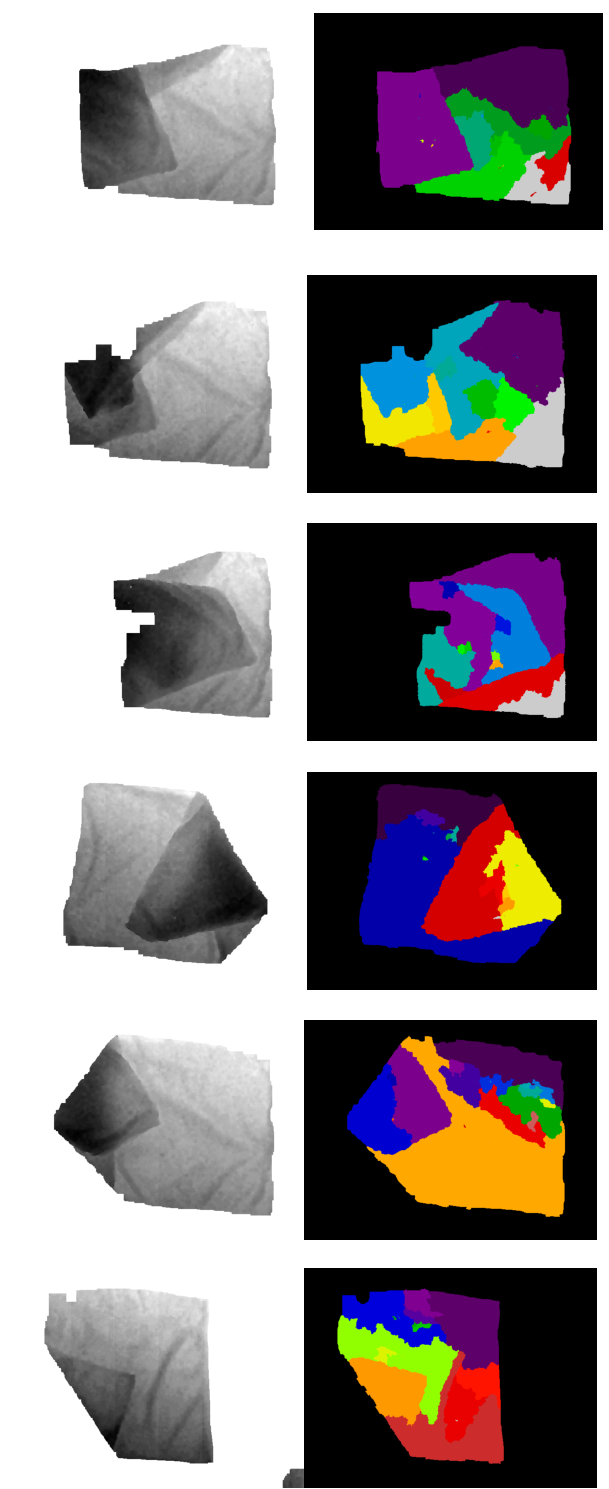
\includegraphics[width=0.38\textwidth]{figures/colour_garment.pdf}
    \caption{On the left side, the grayscale images are shown. The grey level is related to the height of the point as detected by the RGB-D sensor. On the right side, the labeled image returned by watershed algorithm is presented, where each color represents a region of similar height.}
    \label{fig:watershed_labels}
\end{figure}